\documentclass[a4paper, 11pt]{article}

\usepackage[utf8]{inputenc}
\usepackage[english]{babel}

\usepackage{hyperref}

\usepackage{graphicx}
\usepackage{float}

\usepackage{listings}
\usepackage{xcolor}
\definecolor{listinggray}{gray}{0.9}
\definecolor{lbcolor}{rgb}{0.9,0.9,0.9}
\lstset{
	backgroundcolor=\color{lbcolor},
	tabsize=4,    
	language=[GNU]C++,
	basicstyle=\scriptsize,
	upquote=true,
	aboveskip={1.5\baselineskip},
	columns=fixed,
	showstringspaces=false,
	extendedchars=false,
	breaklines=true,
	prebreak = \raisebox{0ex}[0ex][0ex]{\ensuremath{\hookleftarrow}},
	frame=single,
	numbers=left,
	showtabs=false,
	showspaces=false,
	showstringspaces=false,
	identifierstyle=\ttfamily,
	keywordstyle=\color[rgb]{0,0,1},
	commentstyle=\color[rgb]{0.026,0.112,0.095},
	stringstyle=\color[rgb]{0.627,0.126,0.941},
	numberstyle=\color[rgb]{0.205, 0.142, 0.73},
}

\lstset{
	backgroundcolor=\color{lbcolor},
	tabsize=4,
	language=C++,
	captionpos=b,
	tabsize=3,
	frame=lines,
	numbers=left,
	numberstyle=\tiny,
	numbersep=5pt,
	breaklines=true,
	showstringspaces=false,
	basicstyle=\footnotesize,
	%  identifierstyle=\color{magenta},
	keywordstyle=\color[rgb]{0,0,1},
	commentstyle=\color{Darkgreen},
	stringstyle=\color{red}
}

\usepackage{fullpage}

\begin{document}
	\begin{centering}
		\large\textbf{Progress Report: 24/01/2017}\\
		~\\
		Oussama ENNAFII:
		\normalsize MATIS | TITANE \\
		Directors: Cl\'ement Mallet \& Florent Lafarge \\
	\end{centering}


	\section*{Data:}
	
	\begin{itemize}
		\item Available data:
			\begin{itemize}
				\item[-] Bati3D data mostly in 3DS format on: Aix, Annecy, Elancourt, Lambesc, Lyon, Montpellier, Nantes, Paris and Toulouse;
				\item[-] DSM on regions: Toulouse, Elancourt and Nantes; Lambesc needs special application;
				\item[-] BD Ortho (HR) on: Toulouse, Aix, Elancourt, Lambesc and Nantes;
				\item[-] BD topo on: Toulouse.
			\end{itemize}
		\item Misc:
			\begin{itemize}
				\item[-] I need to adapt my script for other XML formats and for tar file handling,
				\item[-] Corrected Bati3D: February, 9th 2017, I am having an appointement with Yannick Couturier (DPR).
			\end{itemize}
	\end{itemize}
	
	\section*{Implementation:}
	I have implemented most of the library to handle 3D data:
	\begin{itemize}
		\item Implemented:
			\begin{itemize}
				\item[-] Reader: 3DS and OFF,
				\item[-] Geomview viewer,
				\item[-] Automated testing;
				\item[-] Algorithms on bricks: area, contour length, affine transformations.
			\end{itemize}
		\item To add:
			\begin{itemize}
				\item[-] Prune Bricks into Buildings and Terrains,
				\item[-] Visualize projections;
			\end{itemize}
		\item To complete:
			\begin{itemize}
				\item[-] Algorithms on bricks: projections (XY and Camera).
				\item[-] Handle KML, Collada and cityGML : I am curently in the process of dicussing this with Antoine Lavenant (D2SI),
				\item[-] Improve logging.
			\end{itemize}
	\end{itemize}
	
	\begin{figure}[H]
		\caption{\label{diag::class} Class diagram.}
		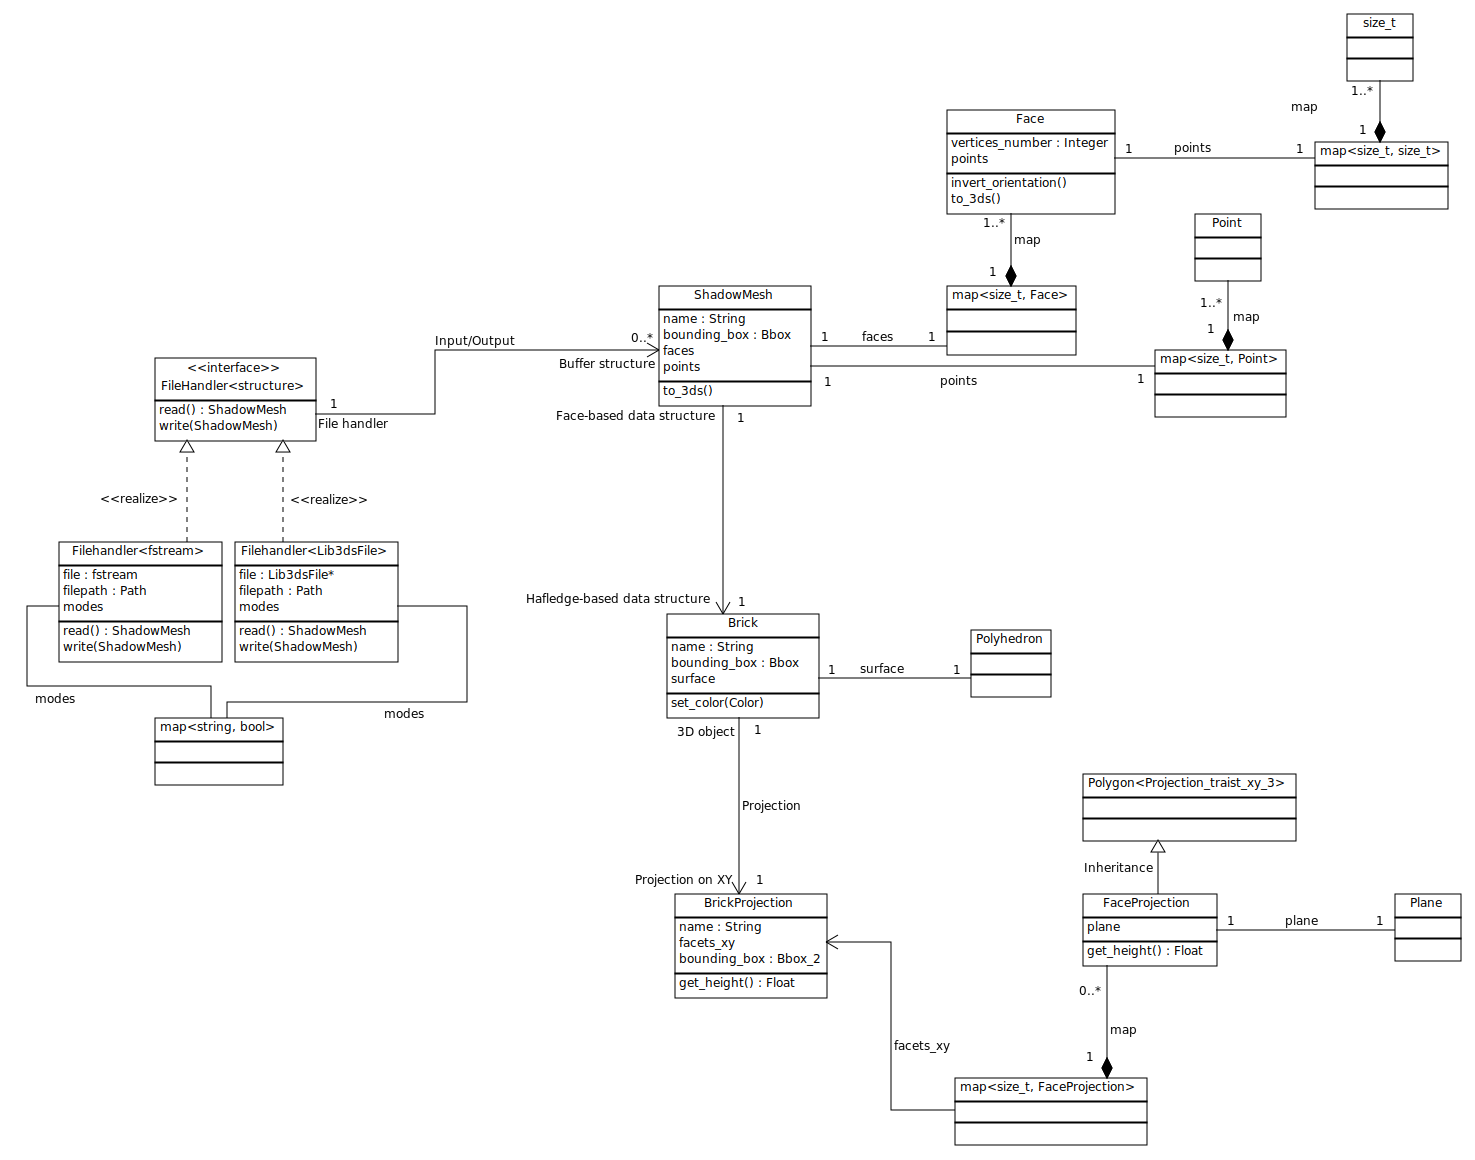
\includegraphics[scale=.3]{images/vectorial/class_diagram.png}
	\end{figure}
	
	\section*{Ideas:}
	There is nothing to report from the last time.
	
	\section*{Results:}
	There is no results to report for now.
	
	\section*{Attachments:}
	
	\begin{itemize}
		\item[-] You can checkout the Code in \href{https://github.com/Ethiy/3DSceneModel}{Github}.
		\item[-] Geomview is "an interactive 3D viewing program for Unix". It is easy enough to visualize $CGAL::Polyhedron\_3$ in Geomview using already implemented $CGAL::Geomview\_stream$. Here is an example of a 3ds file content visualized using Geomview:
		\begin{figure}[H]
			\caption{\label{img::geomview} Santa and Staff visualized using Geomview.}
			\centering 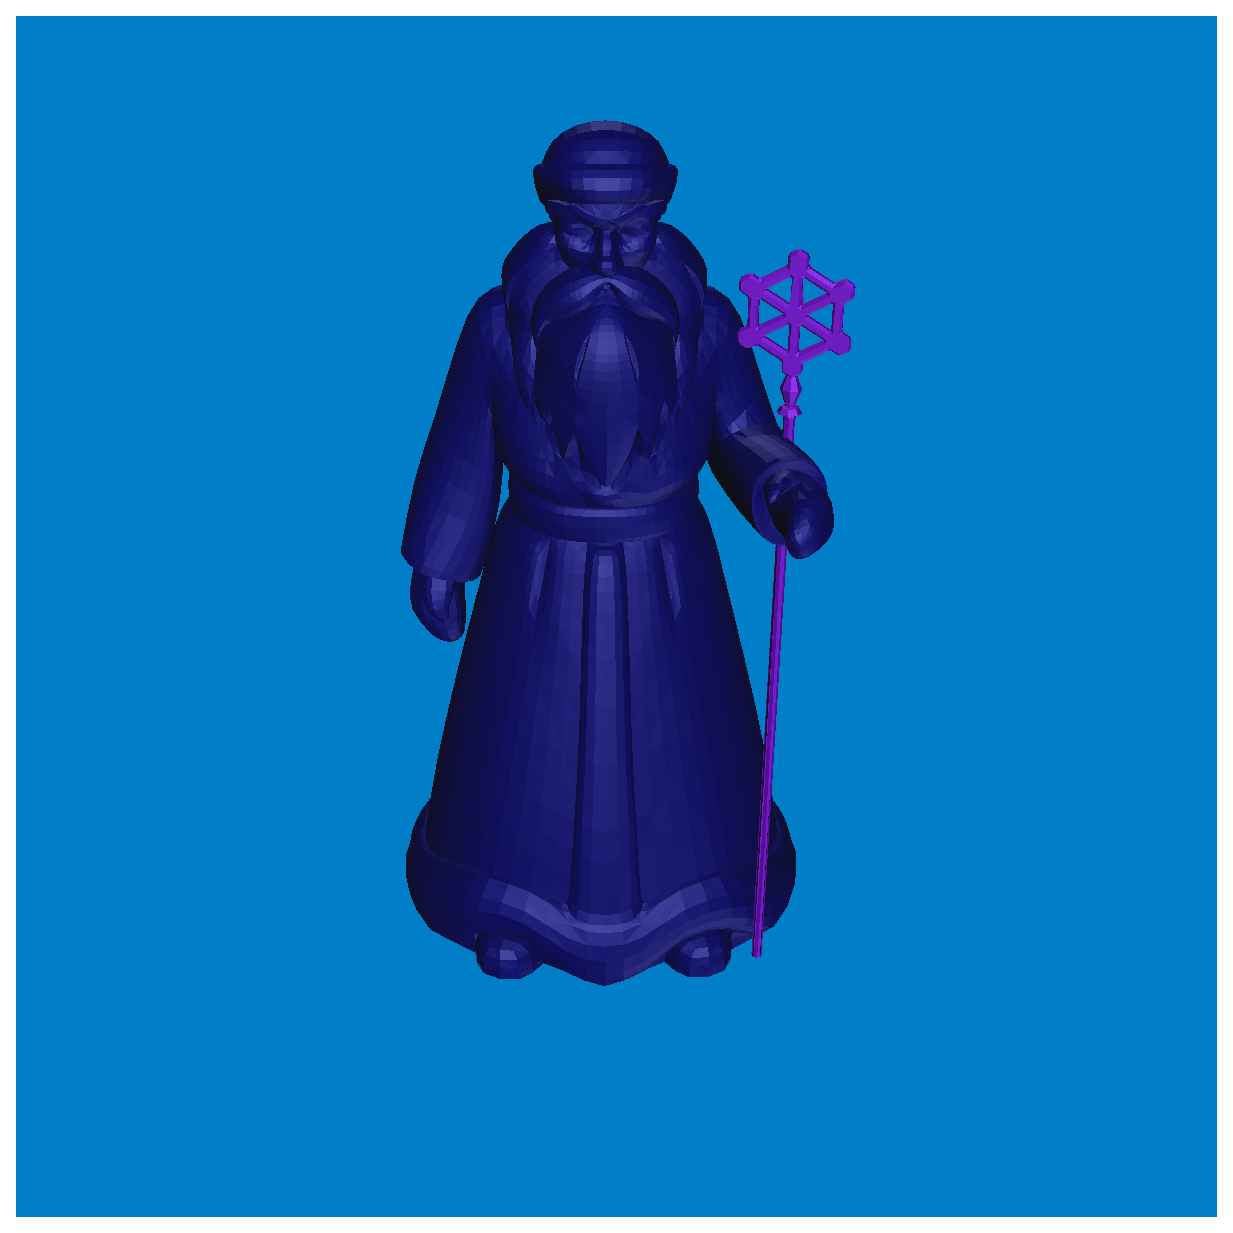
\includegraphics[scale=.4]{images/vectorial/santa.eps}
		\end{figure}
		\item[-] Here after, you can find geometrical definitions for the program:
		\begin{lstlisting}
		#pragma once
		
		#include <CGAL/Homogeneous.h>
		
		#include <CGAL/IO/Color.h>
		
		#include <CGAL/Polyhedron_3.h>
		#include <CGAL/Aff_transformation_3.h>
		
		#include <CGAL/Projection_traits_xy_3.h>
		#include <CGAL/Polygon_2.h>
		
		#include <CGAL/intersections.h>
		
		
		namespace urban
		{
		template <class Refs, class Tag, class Pln>
		struct HalfedgeDS_face_colored : public CGAL::HalfedgeDS_face_base<Refs, Tag, Pln> 
		{
		void set_color(CGAL::Color _color) {color = _color;}
		CGAL::Color get_color(void) {return color;}
		
		CGAL::Color color;
		};
		
		struct Polyhedron_items_colored : public CGAL::Polyhedron_items_3
		{
		template <class Refs, class Traits>
		struct Face_wrapper
		{
		typedef HalfedgeDS_face_colored<Refs, CGAL::Tag_true, typename Traits::Plane_3> Face;
		};
		};
		
		typedef CGAL::Homogeneous<double> Kernel;
		typedef Kernel::Point_3 Point;
		typedef Kernel::Vector_3 Vector;
		typedef Kernel::Plane_3 Plane;
		typedef CGAL::Polyhedron_3<Kernel, Polyhedron_items_colored> Polyhedron;
		typedef Polyhedron::Facet Facet;
		typedef CGAL::Color Color;
		typedef CGAL::Aff_transformation_3<Kernel> Affine_transformation;
		typedef CGAL::Bbox_3 Bbox;
		
		typedef CGAL::Projection_traits_xy_3<Kernel> Projective_traits;
		typedef CGAL::Polygon_2<Projective_traits> Polygon;
		typedef Projective_traits::Point_2 Point_2;
		typedef Projective_traits::Vector_2 Vector_2;
		typedef Projective_traits::Intersect_2 Intersect_2;
		typedef CGAL::Bbox_2 Bbox_2;
		}
		
		\end{lstlisting}
		
	\end{itemize}
	
\end{document}
